\subsection{Sprachsynthese}

\subsubsection*{Benutzeroberfläche}

Erweiterung Inbox um T2S Icon. \\
Erweiterung Admin UI um Checkbox. \\
Zusätzlich Configuration Page mit preferences. \\

\subsubsection*{Konfiguration}

Erweiterung NotificationType um ein boolean Flag für isTextToSpeech.
Wenn Aktiviert, wird Benachrichtigung bei Empfang vorgelesen.

Weiter wird auf dem NotificationType ein Feld version hinzugefügt.
Damit soll die aktuelle Version des NotificationType verfolgt werden.
Wird eine Änderung am NotificationType persisteirt, wird die Version entsprechend angepasst.
Sowohl das Flag isTextToSpeech als auch das version Property werden neu beim Versenden von Benachrichtigungen mitgegeben.

Text To Speech kann auf Client Seite dekativiert werden.
Ist es deaktiviert, werden keine Benachrichtigungen vorgelesen.
Audio Signal, dass Benachrichtung empfangen wurde ertönt aber trotzdem.
Keine zusätzlichen Endpoints am Cloud Service nötig. \\

\begin{figure}[h]
    \centering
    \begin{minipage}[b]{0.75\textwidth}
        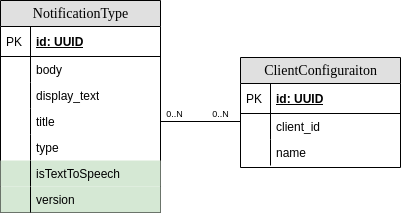
\includegraphics[width=\textwidth]{/home/joshua/FHNW/dev/IP6/IP6_Bachelorarbeit_Bericht_Cloudbasiertes_Praxisrufsystem/src/graphics/diagramms/erd_t2s_v01.drawio}
        \caption{ERD Ausschnitt - Konfiguration Sprachsynthese}
    \end{minipage}
\end{figure}

\clearpage

\subsection*{Anbindung Sprachsynthese Service}

Die Anbindung des Sprachsynthese Service erfolg zentral über den Cloud Service.
Dazu wird der Cloud Service um ein modul Speech erweitert.
Dieses Modul stellt einen Endpoint zur verfügung über den die Sprachdaten zu einer Benachrichtigung abgefragt werden können.
Einziger Parameter für diese Anfrage ist die technische Identifikation des Benachrichtigungstyps der relevanten Benachrichtigung.
Das Speech-Modul kann anhand dieser Identifikation den NotificationType beim Configuration-Modul abholen.
Dem NotificationType kann der Text entonmmen werden, der snytetisiert werden soll.
Dieser Text kann dann an den Sprachsynthese Service gesendet werden.
Das Resultat dieser Anfrage wird als Resultat der Abfrage vom Client zurückgegeben.

\lstinputlisting[caption=SpeechSynthesisController.java,language=java,label={lst:SpeechSynthesisController.java}]{listings/SpeechSynthesisController.java}

Um die Anbindung im Cloud Service vom konkreten Anbieter möglichst unabhängig zu machen, wird die Integration an den Speech Synthese Service über ein Interface abstrahiert.
Soll ein neuer Sprachsyntese Service angebunden werden, muss lediglich dieses Interface für den neuen Service implementiert werden und alles andere kann unberührt bleiben.

\lstinputlisting[caption=SpeechSynthesisService.java,language=java,label={lst:SpeechSynthesisService.java}]{listings/SpeechSynthesisService.java}

Für dieses Projekt wird AWS Polly verwendet.
Dementsprechend wird das SprachSyntheseService Interface für AWS Polly implementiert.
AWS Polly bietet einen Java SDK, welcher die Anbindung ermöglicht.
Dieser SDK bietet alle Klassen die für die Anbindung an AWS Polly nötig sind.
Da im Cloud Service Spring Boot verwendet wird, können die für die Verbindung nötigen Klassen mit einer Spring Config erstellt werden
und dann über Dependency Injection im AwsPollySpeechSynthesis Service verwendet werden.

\lstinputlisting[caption=AwsConfiguration.java,language=java,label={lst:AwsConfiguration.java}]{listings/AwsConfiguration.java}

In der Implementation des Services kann nun über den injezierten AmazonPollyClient eine Abfrage an den Speech Synthesis Service gesendet werden.

\clearpage


\subsection*{Laufzeitsicht}

Empfang und Versenden gleich wie bei IP5.
Benachrichtigung enthält zudem neu Flag ob T2S gebraucht werden soll.
Wenn ja, wird Vorlesen an T2S Service delegiert.

\begin{figure}[h]
    \centering
    \begin{minipage}[b]{0.9\textwidth}
        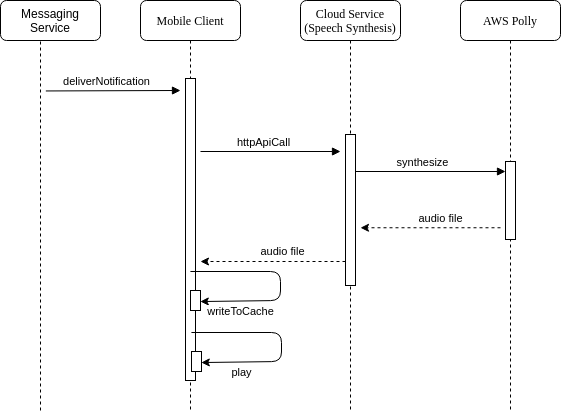
\includegraphics[width=\textwidth]{graphics/diagramms/Sequence_Speech_Synth_V01}
        \caption{Ablauf Benachrichtigung empfangen}
    \end{minipage}
\end{figure}

\clearpage
